% !TEX root = main.tex

\section{聚类}
直观来讲,我们希望“物以类聚”,即同一簇的样本尽可能彼此相似,不同簇的样本尽可能不同。
换言之,聚类结果的簇内相似度(intra-cluster similarity)高,且簇间相似度(inter-cluster similarity)低,这样的聚类效果较好。

性能度量指标:
\begin{itemize}
\item 外部指标
\begin{itemize}
	\item Jaccard系数(Jaccard Coefficient, JC)
	\[JC=\frac{a}{a+b+c}\]
	\item FM指数(Fowlkes and Mallows Index, FMI)
	\[FMI=\sqrt{\frac{a}{a+b}\frac{a}{a+c}}\]
	\item Rand指数(Rand Index, RI)
	\[RI=\frac{2(a+d)}{m(m-1)}\]
\end{itemize}
\item 内部指标:考虑聚类结果的簇划分$\mathcal{C}=\{C_1,C_2,\ldots,C_k\}$
\begin{itemize}
	\item 簇$C_l$内样本间的平均距离
	\[avg(C_l)=\frac{2}{|C_l|(|C_l-1|)}\sum_{1\leq i\leq j\leq |C_l|}dist(x_i,x_j)\]
	\item 簇$C_l$内样本间的最远距离
	\[diam(C_l)=\max_{1\leq i\leq j\leq |C_l|}dist(x_i,x_j)\]
	\item 簇$C_i$与簇$C_j$最近样本间的距离
	\[d_{\min}(C)=\min_{x_i\in C_i,x_j\in C_j}dist(x_i,x_j)\]
	\item 簇$C_i$与簇$C_j$中心点间的距离
	\[d_{cen}(C)=dist(\mu_i,\mu_j)\]
	\item DB指数(Davies-Bouldin Index, DBI):越小越好
	\[DBI=\frac{1}{k}\sum_{i=1}^k\max_{j\ne i}\lrp{\frac{avg(C_i)+avg(C_j)}{d_{cen}(\mu_i,\mu_j)}}\]
	\item Dunn指数(Dunn Index, DI):越大越好
	\[DI=\min_{1\leq i\leq k}\left\{\min_{j\ne i}\lrp{\frac{d_{\min}(C_i,C_j)}{\max_{1\leq l\leq k}diam(C_l)}}\right\}\]
\end{itemize}
\end{itemize}

VDM(Value Difference Metric)可以用于处理无序属性,令$m_{u,a}$表示属性$u$上取值为$a$的样本数,$m_{u,a,i}$表示在第$i$个样本簇中在属性$u$上取值为$a$的样本数,$k$为样本数,则属性$u$上两个离散值$a$与$b$之间的VDM距离为
\[VDM_p(a,b)=\sum_{i=1}^k\left|\frac{m_{u,a,i}}{m_{u,a}}-\frac{m_{u,b,i}}{m_{u,b}}\right|^p\]

\subsection{原型聚类}
给定样本集$D=\{\vx_1,\vx_2,\ldots,\vx_m\}$,Kmeans针对聚类所得簇划分$\mathcal{C}=\{C_1,C_2,\ldots,C_k\}$最小化平方误差
\[MSE=\sum_{i=1}^k\sum_{\vx\in C_i}\norm{\vx-\vmu_i}_2^2\]
其中$\vmu_i$为簇$C_i$的均值向量。
上式一定程度上刻画了簇内样本围绕簇均值向量的紧密程度,$MSE$越小则簇内样本相似度越高。

初始化每个簇的均值向量,不断更新簇划分并重新计算均值,若均值向量均未更新则停止。

\subsection{密度聚类}
此类算法假设聚类结构能通过样本分布的紧密程度来确定。
通常情况下,密度聚类算法从样本密度的角度来考察样本之间的可连接性,并基于可连接样本不断扩展聚类簇来获得最终的聚类结果。

DBSCAN基于一组邻域参数$(\epsilon,MinPts)$来刻画样本分布的紧密程度。
给定数据集$D=\{\vx_1,\vx_2,\ldots,\vx_m\}$,定义以下概念:
\begin{itemize}
	\item $\epsilon$-邻域:$N_{\epsilon}=\{\vx_i\in\mD\mid dist(\vx_i,\vx_j)\leq\epsilon\}$
	\item 核心对象(core object):若$|N_{\epsilon}(\vx_j)|\geq MinPts$,则$\vx_j$是一个核心对象
	\item 密度直达(directly density-reachable):若$\vx_j$位于$\vx_i$的$\epsilon$-邻域中,且$\vx_i$是核心对象,则称$\vx_j$由$\vx_i$密度直达(通常不满足对称性)
	\item 密度可达(density-reachable):对$\vx_i$和$\vx_j$,若存在样本序列$\vp_1,\vp_2,\ldots,\vp_n$,其中$\vp_1=\vx_1$,$\vp_n=\vx_j$且$\vp_{i+1}$由$\vp_i$密度直达,则称$\vx_j$由$\vx_i$密度可达(单侧)
	\item 密度相连(density-connected):对$\vx_i$与$\vx_j$,若存在$\vx_k$使得$\vx_i$与$\vx_j$均由$\vx_k$密度可达,则称$\vx_i$与$\vx_j$密度相连(满足对称性)
\end{itemize}
\begin{figure}[H]
\centering
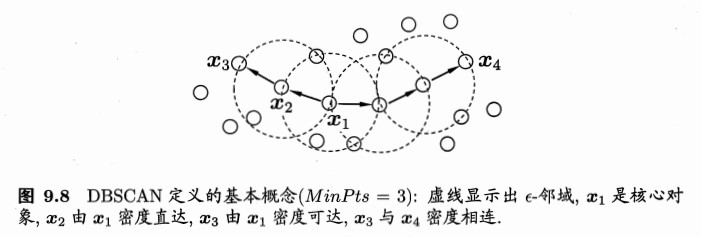
\includegraphics[width=0.8\linewidth]{fig/DBSCAN.jpg}
\end{figure}

进而DBSCAN将“簇”定义为:由\textbf{密度可达关系导出的最大密度相连样本集合},即簇$\mC\subset\mD$是满足以下性质的非空样本子集:
\begin{itemize}
	\item 连接性:$\vx_i\in\mC,\vx_j\in\mC\implies\vx_i$与$\vx_j$密度相连
	\item 最大性:$\vx_i\in\mC$,$\vx_j$由$\vx_i$密度可达$\implies\vx_j\in\mC$
\end{itemize}
实际上,若$\vx$为核心对象,由$\vx$密度可达的所有样本构成的集合$X=\{\vx'\in\mD\mid\vx'\text{由}\vx\text{密度可达}\}$,则$X$为满足连接性与最大性的簇。
注意对于DBSCAN来说,可能存在不属于任何簇的样本,这些样本被认为是噪声(noise)或异常(anomaly)样本。

具体实现可先找出所有的核心对象,然后用队列维护进行扩展。

\subsection{层次聚类}
层次聚类试图在不同层次对数据集进行划分,从而形成树形的聚类结构。数据集划分既可采用“自底向上”的聚合策略,也可采用“自顶向下”的分拆策略。

AGNES算法(自底向上):
首先,将样本中的每一个样本看做一个初始聚类簇,然后在算法运行的每一步中找出距离最近的两个聚类簇进行合并,该过程不断重复,直到达到预设的聚类簇的个数。
这里两个聚类簇$C_i$和$C_j$的距离,可以有3种度量方式:
\begin{itemize}
	\item 最小距离:$d_{\min}(C_i,C_j)=\min_{\vx\in C_i,\vz\in C_j}dist(\vx,\vz)$
	\item 最大距离:$d_{\max}(C_i,C_j)=\max_{\vx\in C_i,\vz\in C_j}dist(\vx,\vz)$
	\item 平均距离:$d_{avg}(C_i,C_j)=\frac{1}{|C_i||C_j|}\sum_{\vx\in C_i}\sum_{\vz\in C_j}dist(\vx,\vz)$
\end{itemize}
\begin{figure}[H]
\centering
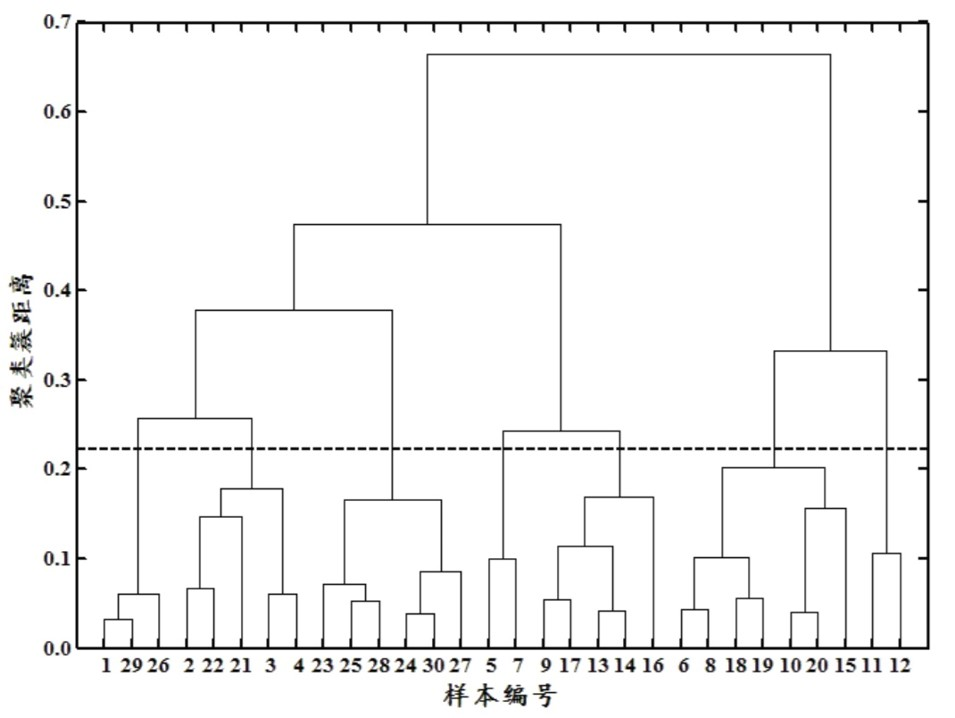
\includegraphics[width=0.8\linewidth]{fig/AGNES.jpg}
\end{figure}